% SPDX-License-Identifier: CC-BY-SA-4.0
%
% Copyright (c) 2020 Philipp Le
%
% Except where otherwise noted, this work is licensed under a
% Creative Commons Attribution-ShareAlike 4.0 License.
%
% Please find the full copy of the licence at:
% https://creativecommons.org/licenses/by-sa/4.0/legalcode

\chapter{Spread Spectrum and Multiple Access}

\begin{refsection}
	
The electromagnetic spectrum is a sparse resource. It must be used as efficient as possible because it is shared with numerous users and applications. However, modern digital communication systems use spread spectrum technologies that occupy a relatively wide frequency band

The purpose of spread spectrum is amongst others:
\begin{itemize}
	\item Immunity against noise and disturbances
	\item Encryption and confidentiality of the communication
	\item Plausible deniability that the communication had ever taken place
	\item Coexistence with other services (multiple access)
\end{itemize}

Especially, the multiple access is an important reason for employing spread spectrum technologies. In modern communication systems, the resource \emph{frequency} is not only allocated to a single user. For example, \ac{LTE} allows many users to access the service with high data rates and low latency. The resource \emph{frequency} must be shared. Efficient medium access relies on spread spectrum to achieve this.

\section{Spread Spectrum}

In the modulation techniques considered so far, are \emph{plain} or \emph{non-spread spectrum}. For the definition of spread spectrum signals, the symbol duration and the transmission bandwidth is investigated.
\begin{itemize}
	\item The signal duration is the amount of time required to convey an information. In digital communication system, an information is a symbol modulated onto a carrier. The signal duration is the symbol period $T_{sym}$.
	\item The signal bandwidth $\Delta f_{sym}$ is the minimum bandwidth required by the receiver to receive the signal. In the case of modulation, it is the \emph{transmission bandwidth}.
\end{itemize}
In the \ac{ASK}, \ac{PSK} and \ac{QAM} modulation of Chapter 5, the signal duration and the bandwidth are inversely proportional.
\begin{equation}
	\Delta f_{sym} = \frac{1}{T_{sym}}
\end{equation}

The product of the bandwidth and the duration -- the \index{time-bandwidth product} \textbf{time-bandwidth product} -- is constantly $1$.\footnote{This is the ideal case. For real implementations, the constant may differ from $1$ depending on the modulation technique. However, it will be close to $1$.}
\begin{equation}
	T_{sym} \cdot \Delta f_{sym} = 1
\end{equation}

\paragraph{Time-Bandwidth Product.}

The time-bandwidth product is used for the definition of spread spectrum:
\begin{definition}{Spread spectrum}
	The time-bandwidth product of \index{spread spectrum} \textbf{spread spectrum} signals is significantly greater than $1$.
	\begin{equation}
		T_{sym} \cdot \Delta f_{sym} \gg 1
	\end{equation}
\end{definition}

Typically, this means that the bandwidth $\Delta f_{sym}$ is increased while the symbol duration and thereby the symbol rate is kept constant.
\begin{itemize}
	\item The symbol sequence (time-bandwidth product of $1$) is altered in a way which distributes the signal power over a wider frequency band. This process is called \index{spreading} \textbf{spreading}.
	\item The inverse process is \index{despreading} \textbf{despreading}. The original symbol sequence is reconstructed from the wide-band spread spectrum signal.
\end{itemize}

\begin{figure}[H]
	\centering
	\begin{tikzpicture}
		\begin{axis}[
			height={0.15\textheight},
			width=0.8\linewidth,
			scale only axis,
			xlabel={$\omega$},
			ylabel={$|\mathrm{S}_{XX}|$},
			%grid style={line width=.6pt, color=lightgray},
			%grid=both,
			grid=none,
			legend pos=north east,
			axis y line=middle,
			axis x line=middle,
			every axis x label/.style={
				at={(ticklabel* cs:1.05)},
				anchor=north,
			},
			every axis y label/.style={
				at={(ticklabel* cs:1.05)},
				anchor=east,
			},
			xmin=0,
			xmax=10.5,
			ymin=0,
			ymax=1.2,
			xtick={0},
			xticklabels={0},
			ytick={0},
			axis x discontinuity=parallel,
		]
			\addplot[blue, smooth] coordinates {(4.6,0) (4.7,0.02) (4.8,0.2) (4.9,0.71) (5,1) (5.1,0.71) (5.2,0.2) (5.3,0.02) (5.4,0)};
			\addlegendentry{Narrow-band signal};
			\addplot[red, smooth] coordinates {(2,0) (2.5,0.01) (3,0.05) (5,0.05) (7,0.05) (7.5,0.01) (8,0)};
			\addlegendentry{Spread spectrum signal};
		\end{axis}
	\end{tikzpicture}
	\caption[PSD of a narrow-band and spread spectrum signal]{\acs{PSD} of a narrow-band and spread spectrum signal. Both signals carry the same information and have the equal power. The narrow-band signal concentrates the whole signal power in a narrow frequency band. In contrast, the spread spectrum signal distributes the signal power over a wide frequency band.}
\end{figure}

\paragraph{Noise-like Signal.}

The signal power remains constant while the signal is spread.
\begin{itemize}
	\item The \ac{PSD} is reduced.
	\item But, the \ac{PSD} is integrated over a wider frequency range.
	\item The overall power remains constant.
\end{itemize}

The \ac{PSD} of the spread spectrum signal is flat in approximation.
\begin{itemize}
	\item The flat \ac{PSD} resembles the \ac{PSD} of noise.
	\item Spread spectrum signal are therefore \emph{noise-like}.
\end{itemize}

A third party who has no knowledge of neither the existence of the spread spectrum signal nor the technology used cannot detect the signal.
\begin{itemize}
	\item The spread spectrum signal looks like noise or a wide-band disturbance from the view of the receiver which does not participate in the communication.
	\item This circumstance can be used to conceal the existence of the signal (plausible deniability of its existence).
\end{itemize}

\paragraph{Despreading.}

\index{despreading} Despreading reconstructs the symbols -- and thereby the data -- from the spread spectrum signal.
\begin{itemize}
	\item The spreading is reversed.
	\item The symbols (time-bandwidth product of $1$) are reconstructed. This can be seen like re-concentrating the spread signal power in a narrow-band symbol sequence.
	\item The disturbances which are uncorrelated to the spread spectrum signal are converted into the wide-band noise with a low \ac{PSD}.
	\begin{itemize}
		\item The wide-band noise floor (like thermal noise or quantization noise) remains wide-band.
		\item Strong but narrow-band disturbing signals (like other users of the electromagnetic spectrum) are spread to low-\acs{PSD} wide-band noise during the despreading. The \ac{SNR} is increased by spreading the signal power of the disturbance.
	\end{itemize}
\end{itemize}

\todo{Despreading in frequency-domain, suppression of noise and disturbances}

\subsection{Direct-Sequence Spread Spectrum}

A simple method for increasing the bandwidth systematically re-encoding the symbols using new symbols at a higher symbol rate.
\begin{itemize}
	\item The input symbols are at the rate of $f_{sym}$.
	\item The \emph{spreading} is achieved by re-encoding each symbol by $M$ new symbols, called \index{chip} \textbf{chips}.
	\item After re-encoding, the rate of the new symbols -- the \emph{chips} -- is $f_{chp}$. $f_{chp}$ is the \index{chip rate} \textbf{chip rate}.
	\item $M$ is the \index{spreading factor} \textbf{spreading factor}.
	\begin{equation}
		M = \frac{f_{chp}}{f_{sym}}
	\end{equation}
\end{itemize}

\begin{example}{\acs{IEEE} 802.11b}
	\acs{IEEE} 802.11b is an early \ac{WLAN} standard from 1999, defining data rates of \SI{1}{Mbit/s} to \SI{11}{Mbit/s}.\footnote{In comparison to that modern \ac{WLAN} standards like \acs{IEEE} 802.11ax have data rates of several \si{Gbit/s}. But they use other spread spectrum technologies.} Usually, the data rate is proportional to the transmission bandwidth. But, \acs{IEEE} 802.11b uses \ac{DSSS} to implement an adaptive data rate whilst retaining a constant bandwidth (approximately \SI{22}{MHz}).
	
	\begin{figure}[H]
		\centering
		\begin{circuitikz}
			\node[mixer](Spreader){};
			\node[draw,block,below=1.5cm of Spreader](Code){Code\\ generator};
			\node[draw,block,right=3cm of Spreader](Mod){\acs{BPSK}\\ modulator};
			
			\node[above=3mm of Spreader,align=center]{Multiplier as\\ the spreader};
			
			\draw[-o] (Spreader.west) node[inputarrow]{} -- ++(-1cm,0) node[left,align=right]{Input data\\ at $f_{sym}$};
			\draw (Code.north) -- node[midway,right,align=left]{Spreading code\\ at $f_{chip}$} (Spreader.south) node[inputarrow,rotate=90]{};
			\draw (Spreader.east) -- node[midway,above,align=center]{Chip\\ sequence} (Mod.west) node[inputarrow]{};
			\draw (Mod.east) -- ++(1cm,0) node[inputarrow]{} node[right,align=left]{Baseband\\ signal};
		\end{circuitikz}
		\caption{Simplified spreading and \acs{PSK} modulation signal chain of an \acs{IEEE} 802.11b conforming transmitter}
	\end{figure}

	Data is represented by bits. At a data rate of $f_{sym} = \SI{1}{Mbit/s}$, the data is spread by a factor $M = 11$. The data symbols are multiplied by the \emph{spreading code}. Because of the multiplication, the same block symbol as the mixer is used. The code has a \emph{chip rate} of $f_{chp} = M f_{sym} = \SI{11}{Mchp/s}$.\footnote{Physically, the units \si{bit} and \si{chp} are dimension-less. Therefore, $\SI{1}{Mbit/s} = \SI{1}{Mchp/s} = \SI{1}{MHz}$. However, the units shall refer to the quantity being considered.}
	
	\vspace{0.5em}
	
	For $M = 11$, the \index{Barker code} \textbf{Barker code} with $\vect{C}_{11} = \left[+1, +1, +1, -1, -1, -1, +1, -1, -1, +1, -1\right]$ is used as the spreading code. Let's consider a bit stream of $(10)_2$ as th data, which is encoded as the symbols $\vect{D} = \left[-1, +1\right]$. The spread sequence is:
	\begin{equation}
		\begin{split}
			\vect{S} &= \vect{D} \otimes \vect{C}_{11} \\
			 &= \left[\underbrace{-1, -1, -1, +1, +1, +1, -1, +1, +1, -1, +1}_{\text{Spread symbol } -1},\right. \\ &\qquad \left.  \underbrace{+1, +1, +1, -1, -1, -1, +1, -1, -1, +1, -1}_{\text{Spread symbol } +1}\right]
		\end{split}
	\end{equation}
	
	The \emph{chip sequence} $\vect{S}$ is at a rate of \SI{11}{Mchp/s}. In this case, the \emph{chip} have two discrete states $-1$ or $+1$. They can be modulated by a \ac{BPSK} modulator. It baseband is then mixed to the \ac{RF} band of \SI{2.4}{GHz} using an IQ modulator.
	
	\vspace{0.5em}
	
	At a data rate of \SI{11}{Mbit/s}, the data is \underline{not} spread ($M = 1$). The spreading code is $\vect{C}_{1} = \left[+1\right]$. The \emph{chip rate} equals the data bit rate. The \emph{chip rate} remains constant at \SI{11}{Mchp/s}.
	
	\vspace{0.5em}
	
	\textbf{Why adaptive data rate?} Spreading by $M = 11$ increases the \ac{SNR}. Each symbol is effectively repeated 11 times. This circumstance can be used to achieve a processing gain and increase noise immunity. The higher data rate at a lower spreading factor of $M = 1$ comes at the drawback of decreased noise immunity.
\end{example}

The \index{direct-sequence spread spectrum} \textbf{\acf{DSSS}} spreads the symbols by multiplying each data symbol with the whole spreading code.
\begin{itemize}
	\item The data symbol sequence is represented by the vector $\vect{D}$. A single data symbol is $D_n$.
	\item The data comes at the rate of $f_{sym}$.
	\item The code sequence is represented by the $M$-dimensional vector $\vect{C}_M$. $M$ is the length of the code. A single chip of the code is $C_m$.
	\item The code repeats at $f_{sym}$. The rate of the single code chips is $f_{chp} = M f_{sym}$.
\end{itemize}
The process of multiplying each data symbol $D_n$ with the whole code sequence $\left[C_0, C_1, \dots, C_{M-1}\right]$ is represented by the \index{Kronecker product} \textbf{Kronecker product} $\otimes$. \nomenclature[Fk]{$\otimes$}{Kronecker product}
\begin{equation}
	\begin{split}
		\vect{S} &= \vect{D} \otimes \vect{C}_{M} \\
		S_{n M + m} &= D_n \cdot C_m \qquad \forall 0 \leq m < M
	\end{split}
\end{equation}
$\vect{S}$ is the sequence of output chips -- the \emph{spread spectrum signal}. The chips in $\vect{S}$ are at the chip rate of $f_{chp} = M f_{sym}$.

\begin{figure}[H]
	\centering
	\begin{circuitikz}
		\node[draw,block](Spreader){Spreader\\ $\vect{D} \otimes \vect{C}_{M}$};
		\node[draw,block,below=1.5cm of Spreader](Code){Code\\ generator};
		\node[draw,block,right=2.5cm of Spreader](Mod){Modulation\\ (\acs{BPSK}, \acs{QPSK},\\ \acs{QAM}, ...)};
		
		\draw[-o] (Spreader.west) node[inputarrow]{} -- ++(-1cm,0) node[left,align=right]{Input symbol\\ sequence $\vect{D}$};
		\draw (Code.north) -- node[midway,right,align=left]{Spreading\\ code $\vect{C}_{M}$} (Spreader.south) node[inputarrow,rotate=90]{};
		\draw (Spreader.east) -- node[midway,above,align=center]{Chip\\ sequence\\ $\vect{S}$} (Mod.west) node[inputarrow]{};
		\draw (Mod.east) -- ++(1cm,0) node[inputarrow]{} node[right,align=left]{Baseband\\ signal};
	\end{circuitikz}
	\caption{Abstract \acs{DSSS}}
	\label{fig:ch07:abstract_dsss}
\end{figure}

Figure \ref{fig:ch07:abstract_dsss} depicts an abstract view on \ac{DSSS}. The \emph{spreading code} is a \index{pseudorandom code} \textbf{pseudorandom code}.
\begin{itemize}
	\item The code is generated by an algorithm and is thereby predictable if the algorithm is known.
	\item For a receiver that does not know the code generation algorithm, the code sequence is random. It is noise-like.
	\item \textit{The fact, that the code must be known to the receiver, can be used to implement data encryption.}
\end{itemize}

Example usage of \ac{DSSS}:
\begin{itemize}
	\item \acs{IEEE} 802.11b specification for \ac{WLAN}
	\item \ac{GPS}
\end{itemize}

\subsection{Frequency-Hopping Spread Spectrum}

Example usage of \ac{FHSS}:
\begin{itemize}
	\item \acs{IEEE} 802.15.1 (Bluetooth)
\end{itemize}

\subsection{Time-Hopping Spread Spectrum}

Example usage of \ac{THSS}:
\begin{itemize}
	\item \ac{UWB} systems conforming to \acs{IEEE} 802.15.4
\end{itemize}

\subsection{Symbol Reconstruction}

\todo{Processing Gain}

\todo{Reception under noise}

\todo{Cross-correlation}

\section{Multi-carrier Modulation}

\todo{OFDM}

\section{Multiple Access}

\todo{Multiplexing}

\todo{Sharing Resources}

\subsection{Space-Division Multiple Access}

\subsection{Time-Division Multiple Access}

\subsection{Frequency-Division Multiple Access}

\subsection{Code-Division Multiple Access}

\subsection{Orthogonal Frequency-Division Multiple Access}

\section{Orthogonal Codes}

\nocite{ipatov2005}

\phantomsection
\addcontentsline{toc}{section}{References}
\printbibliography[heading=subbibliography]
\end{refsection}

